%%%%%%%%%%%%%%%%%%%%%%%%%%%%%%%%%%%%%%%%%%%%%%%%%%%%%%%%%%%%%%%%%%%%%%
%
% Documentation for the tikzducks package
% A package to bring rubber ducks into tikz
% Maintained by samcarter
%
% Project repository and bug tracker:
% https://github.com/samcarter/tikzducks
%
% Released under the LaTeX Project Public License v1.3c or later
% See http://www.latex-project.org/lppl.txt
%
%%%%%%%%%%%%%%%%%%%%%%%%%%%%%%%%%%%%%%%%%%%%%%%%%%%%%%%%%%%%%%%%%%%%%%
\documentclass[parskip=half]{scrartcl}

% packages %%%%%%%%%%%%%%%%%%%%%%%%%%%%%%%%%%%%%%%%%%%%%%%%%%%%%%%%%%%
\usepackage[T1]{fontenc}  
\usepackage[utf8]{inputenc}    
\usepackage[english]{babel}
\usepackage[bitstream-charter]{mathdesign}
\usepackage{tikzducks}
\usetikzlibrary{ducks,3d}
\usepackage[most]{tcolorbox}
\usepackage[paper=a4paper,margin=3cm,foot=2cm]{geometry}
\usepackage{url}
\usepackage{xspace}
\usepackage{scrlayer-scrpage} 
\usepackage{marvosym}
\usepackage{fontawesome}
\usepackage[hang,flushmargin,bottom]{footmisc}
\usepackage{imakeidx}
\usepackage[colorlinks=true,breaklinks=true,urlcolor=duckblue,linkcolor=duckblue,citecolor=duckblue,filecolor=duckblue]{hyperref}

% macros %%%%%%%%%%%%%%%%%%%%%%%%%%%%%%%%%%%%%%%%%%%%%%%%%%%%%%%%%%%%%
\newcommand{\CTAN}{\textsc{CTAN}\xspace}
\newcommand{\TikZ}{Ti\emph{k}Z\xspace}
\newcommand{\tikzducks}{Ti\emph{k}Zducks\xspace}
\newcommand{\miktex}{MiK\TeX\xspace}
\newcommand{\texlive}{\TeX{}Live\xspace}

% customisation %%%%%%%%%%%%%%%%%%%%%%%%%%%%%%%%%%%%%%%%%%%%%%%%%%%%%%
\definecolor{duckblue}{RGB}{0,70,140}
\addtokomafont{sectioning}{\color{duckblue}}
\addtokomafont{date}{\normalsize}
\addtokomafont{author}{\normalsize}
\setlength{\footnotemargin}{0.7em}

\lstdefinestyle{duckstyle}{%
  language={[latex]TeX},
  tabsize=2,
  breaklines,
  basicstyle=\footnotesize\ttfamily,
  commentstyle={\color{green!50!black}\slshape}, 
  columns=fullflexible,
  emphstyle=\color{orange!70!black},
  emph=[1]{water,body,head,eye,pupil,bill,grumpy,tshirt,jacket,tie,cape,shorthair,longhair,crazyhair,recedinghair,eyebrow,beard,glasses,sunglasses,alien,hat,cap,santa,chef,cheese,graduate,tassel,beret,crown,unicorn,icecream,flavoura,flavourb,flavourc,book,bookcolour,signpost,signcolour,signback,magichat,magicstars,magicwand,witch,cricket,rollingpin,lightsaber,torch,cake,pizza,hockey,baguette,wing,football,mask,bunny,inear,necklace,milkshake,wine,peakedcap,prison,tophat,speech,bubblecolour,think,buttons,sheep,squareglasses,tail,basket,easter,egga,eggb,eggc,mohican,mullet,horsetail,darthvader,crozier,queencrown,kingcrown,wing,laughing,parrot,stethoscope,niuqelrah,harlequin,neckerchief,woggle,snowduck,invisible,strawhat,ribbon,vampire,parting,crystalball,helmet,shovel,pickaxe,bowtie,lapel,umbrella,umbrellaclosed,handbag,cocktail,viking,devil,aodai,conicalhat,overleaf,sailor},
  texcsstyle=*\color{duckblue}\bfseries,
  keywordstyle=\color{red!60!black}\bfseries,
  morekeywords={tikzpicture,picture,scope,patterns,calc,pgfinterruptboundingbox},
  moretexcs={duck,picduck,path,definecolor,duckpathjacket,duckpathbody,duckpathgrumpybill,duckpathbill,duckpathtshirt,duckpathcape,duckpathshorthair,duckpathlonghair,duckpathcrazyhair,duckpathrecedinghair,duckpathcrown,scalebox,foreach,node,draw,PassOptionsToPackage,usetikzlibrary,selectcolormodel,colorlet,insignia,stripes,color,includegraphics,mcap,setboardfontcolors,setboardfontencoding,WhiteQueenOnWhite,WhiteKingOnWhite,superstripes,shuffleducks,randuck,randomhead,randomaccessories,duckpathmohican,duckpathmullet,duckpathqueencrown,duckpathkingcrown,duckpathdarthvader,duckpathhorsetail,tikzset,duckpathwing,shade,duckhookbackground,duckhookbody,duckhookclothing,duckhookhair,duckhookhat,duckhookforeground},
  delim ={[s][\ttfamily\color{green!50!black}]{$}{$}},
  moredelim=[is][\footnotesize\ttfamily\color{orange!70!black}]{|}{|},
  index=[1][emph]
}

\tcbset{%
  colframe=duckblue,
  arc=2mm,
  fonttitle=\bfseries,
  sidebyside,
  listing options={style=duckstyle},
  center lower,
  righthand width=6.5cm,
  bottom=0pt, 
  top=0pt,
  before lower={%
    \setlength{\parskip}{0.5cm}%
    \spaceskip=5\fontdimen2\font%
  },
}

\lstset{style=duckstyle}
\pgfkeys{/duck/|stripes|/.style={stripes={#1}}}

\pgfmathsetseed{2}
\setlength{\footheight}{41pt}
\newlength{\duckoffset}

\cfoot{%
  \tikzset{external/export=false}%
  \shuffleducks
  \begin{tikzpicture}[scale=0.5] 
      \duck[signpost=\scalebox{0.6}{\thepage},\randomhead]
  \end{tikzpicture}
} 
\pagestyle{scrheadings}
\indexsetup{firstpagestyle=scrheadings}
\makeindex[columns=3]

\usetikzlibrary{external}
\ifnum\pdfshellescape=1
  \tikzexternalize[prefix=./tikzducks-doc-figures/]
\fi

% meta %%%%%%%%%%%%%%%%%%%%%%%%%%%%%%%%%%%%%%%%%%%%%%%%%%%%%%%%%%%%%%%
\title{The \texorpdfstring{\tikzducks}{tikzducks} package}
\subtitle{using ducks in \TikZ}
\author{%
  \texorpdfstring{\texttt{samcarter} (alias 
    \tikzset{external/export=false}%
    \begin{tikzpicture}[scale=0.3,baseline=3pt]
      \duck[body=yellow!50!brown!50!white,
          longhair=red!50!brown, 
          jacket=blue!50!black]
    \end{tikzpicture})\\[0.8em]
    \url{https://github.com/samcarter/tikzducks}\\
    \url{https://www.ctan.org/pkg/tikzducks}
  }{samcarter}}
\date{Version v1.4 \textendash{} 2020/04/22}

\begin{document}
\maketitle
\thispagestyle{scrheadings}

\section{Introduc(k)tion}
\label{intro}

Rubber ducks can be made of latex, but can they also be made with \LaTeX? Yes! The \tikzducks package is a \LaTeX{} package for rubber ducks to be used in \TikZ pictures. 
This project is a continuation of \href{tex.stackexchange.com/a/347458/36296}{How can we draw a duck?}.

This package is work in progress (and will probably never be really finished as there is an infinite amount of things which could be added), therefore I would be happy to hear your feedback and ideas how to improve the package. 
The head version of the source code can be found on \url{github.com/samcarter/tikzducks}, including a bug tracker -- please make constructive use of it! A more stable package version can be found on \CTAN (\url{www.ctan.org/pkg/tikzducks}) and is included in both \miktex and \texlive as \tikzducks. If you seek any other assistance (not bug reports/feature requests), I suggest asking a question at \url{topanswers.xyz/tex}.

\subsection{Acknowledgements}

Without the friendly and helpful community of \TeX{} users this package would not exist. I would like to thank a few fellow users in particular:

First of all 
%
Carla Maggi for pointing out the overwhelming need of having a \tikzducks package and valuable contribution to the package code, in particular the \hyperref[sec:footballducks]{football ducks},
%
Paulo Cereda for his contagious enthusiasm for ducks (\emph{Quack!}) and
%
Ulrike Fischer for her useful \TikZ advices and contributions to the package and coming to rescue for keyword highlighting in the package documentation.

Many other users contributed to this package (in random order):
%
Enrico Gregorio helped to implement the \lstinline|\tikzset{}| interface which makes it much easier to adjust the properties of the ducks to fit the user needs,
% 
Andrew Stacey contributed the \TikZ Library ``ducks'',
%
Symbol~1 solved a few problems with default key values,
%
Mihikma created the duck's beard,
%
Yudai Nakata helped with problems of \lstinline|\pdfrandomseed|,
%
@marmot for his seemingly infinite knowledge of \TikZ which he shared with the world    
%
and last but not least my thanks go to Martin Schr\"oder for his feedback to the code review.

\pagebreak
The ducks mostly consist of basic geometric shapes drawn in \TikZ. Some of the more complex shapes (e.g.\ the different hair styles) are first drawn in \texttt{inkscape} (\url{https://inkscape.org}) and then exported to \TikZ paths using the \texttt{SVG to TikZ/PGF} extension (\url{https://github.com/kjellmf/svg2tikz}).

\subsection{Dependencies}

The \tikzducks package loads \TikZ, which in turn loads the \lstinline|xcolor| package (amongst others). If you require one of these packages to be loaded with some option, please consider loading it yourself before the \tikzducks package or use, e.g.

\begin{lstlisting}[morekeywords={xcolor,svgnames}]
  \PassOptionsToPackage{svgnames}{xcolor}
\end{lstlisting}
It also uses the \lstinline|\usetikzlibrary{patterns}| and \lstinline|\usetikzlibrary{calc}|. 

\subsection{License}

Copyright \raisebox{0.2em}{\tiny\fontfamily{cmr}\selectfont\textcopyright}
\texttt{samcarter}. Permission is granted to copy, distribute and\slash or modify this software under the terms of the LaTeX project public licence, version 1.3c or later \url{http://www.latex-project.org/lppl.txt}.

The shown example ducks are purely fictional characters, any resemblance to real ducks or persons is purely coincidental and no copyright infringement is intended.

\section{Usage}

The basic usage is fairly simple, to draw a duck:
\begin{tcblisting}{title={Basic duck}}
\begin{tikzpicture}
  \duck
\end{tikzpicture}
\end{tcblisting}

To customise this basic duck, the package uses \lstinline|pgf| keys. For almost all parts the colour can be changed using \lstinline|<shape name>=<colour name>|. For example to change the colour of the duck:
\begin{tcblisting}{title={Blue duck}}
\begin{tikzpicture}
  \duck[body=blue]
\end{tikzpicture}
\end{tcblisting}

If the keyword consists of multiples words, it works both with and without spaces. In the following usually the version without spaces is given. 

\clearpage
In addition to the keys defined in this package, all usual \TikZ and \lstinline|pgf| keys can also be used. For example if the size of the ducks should be changed or shifted:

\begin{tcblisting}{title={Scaled duck and \emph{The Ugly Duckling}},  righthand width=3cm}
\begin{tikzpicture}[scale=0.6]
  \duck
  \duck[xshift=90pt, scale=.3, yshift=150pt]
  \duck[xshift=60pt, scale=.3, yshift=100pt]
  \duck[body=gray!50!white,head=gray!50!white,
    xshift=80pt, scale=.3, yshift=50pt]
\end{tikzpicture}
\end{tcblisting}

To make the usage easier for the \TikZ-savvy users, Andrew Stacey contributed a \TikZ library. It can be loaded with \lstinline|\usetikzlibrary{ducks}|. In addition to the normal functionality of the \tikzducks package, the ducks are now also available as \lstinline|pic|. A short example:

\begin{tcolorbox}[title={\TikZ library ``ducks''}]
\begin{lstlisting}[morekeywords={ducks,duck,standalone,tikz,document}]
\documentclass{standalone}

\usepackage{tikz}
\usetikzlibrary{ducks}

\begin{document}

\begin{tikzpicture}
\draw (0,0) pic[
    duck/water=green,
    duck/alien,
  ] {duck};
\draw (4,0) pic[
    scale=1.4,
  ] {duck};
\end{tikzpicture}

\end{document}
\end{lstlisting} 

\tcblower
\begin{tikzpicture}
\draw (0,0) pic[
    duck/water=green,
    duck/alien,
  ] {duck};
\draw (2,1) pic[
    scale=1.4,
  ] {duck};
\end{tikzpicture}
\end{tcolorbox}

For everybody suffering from anatidaephobia, there is also a special option to not draw the duck: 
\begin{tcblisting}{title={Invisible duck}}
\begin{tikzpicture}
  \duck[invisible]
\end{tikzpicture}
\end{tcblisting}

This can also be useful to recycle some of the accessories presented in \ref{sec:accessories}.

\clearpage
For the \TeX{} purists, there is also a picture mode variant:

{
\setlength{\unitlength}{0.6mm}
\begin{tcblisting}{title={\texttt{picture} mode duck}}
\begin{picture}(42,44)
  \picduck
\end{picture}
\end{tcblisting}
}

\subsection{Body parts}

The various parts of the duck can also be coloured independently, i.e.\ \lstinline|body|, \lstinline|head| or \lstinline|bill|:

\begin{tcblisting}{title={Harlequin duck}}
\begin{tikzpicture}
  \duck[body=yellow,
    head=yellow!50!orange, 
    bill=red,
    eye=green]
\end{tikzpicture}
\end{tcblisting}

Furthermore using the keywords \lstinline|grumpy|, \lstinline|laughing| or \lstinline|parrot| the shape of the bill can be changed:

\begin{tcblisting}{title={Grumpy duck}}
\begin{tikzpicture}
  \duck[grumpy]
\end{tikzpicture}
\begin{tikzpicture}
  \duck[grumpy, bill=cyan]
\end{tikzpicture}
\end{tcblisting}

\begin{tcblisting}{title={Laughing duck}}
\begin{tikzpicture}
  \duck[laughing]
\end{tikzpicture}
\begin{tikzpicture}
  \duck[laughing, bill=red]
\end{tikzpicture}
\end{tcblisting}

\begin{tcblisting}{title={Parrot duck}}
\begin{tikzpicture}
  \duck[parrot]
\end{tikzpicture}
\begin{tikzpicture}
  \duck[parrot, bill=blue]
\end{tikzpicture}
\end{tcblisting}


\subsection{Hair styles}

Some duck also like to have nice hair cuts, several different hair styles are available:

\begin{tcblisting}{title={Long hair duck}}
\begin{tikzpicture}
  \duck[longhair]
\end{tikzpicture}
\end{tcblisting}

\begin{tcblisting}{title={Short hair duck}}
\begin{tikzpicture}
  \duck[shorthair]
\end{tikzpicture}
\end{tcblisting}

\begin{tcblisting}{title={Parting hair duck}}
\begin{tikzpicture}
  \duck[parting]
\end{tikzpicture}
\end{tcblisting}

\begin{tcblisting}{title={Crazy hair duck}}
\begin{tikzpicture}
  \duck[crazyhair]
\end{tikzpicture}
\end{tcblisting}

\begin{tcblisting}{title={Receding hair duck}}
\begin{tikzpicture}
  \duck[recedinghair]
\end{tikzpicture}
\end{tcblisting}

\begin{tcblisting}{title={Mohican duck}}
\begin{tikzpicture}
  \duck[mohican]
\end{tikzpicture}
\end{tcblisting}

\begin{tcblisting}{title={Mullet duck}}
\begin{tikzpicture}
  \duck[mullet]
\end{tikzpicture}
\end{tcblisting}

And of course the colour of each hair style can be adjusted:
\begin{tcblisting}{title={Coloured hair duck}}
\begin{tikzpicture}
  \duck[longhair=teal]
\end{tikzpicture}
\end{tcblisting}

Eyebrows and a beard are also part of the package. The colour choice is more tricky for them -- if a colour is explicitly specified (\lstinline|eyebrow=<colour name>| or \lstinline|beard=<colour name>|) this colour is of course used, but if no colour is given, it first falls back to the hair colour and only if the duck does not have any hairs, the default colour is applied.

\begin{tcblisting}{title={Eye brow duck}}
\begin{tikzpicture}
  \duck[eyebrow]
\end{tikzpicture}
\begin{tikzpicture}
  \duck[longhair=blue,eyebrow]
\end{tikzpicture}

\begin{tikzpicture}
  \duck[crazyhair=red,eyebrow=blue]
\end{tikzpicture}
\end{tcblisting}

\addtocounter{footnote}{1}
\begin{tcblisting}{title={Beard duck$^{\thefootnote}$}}
\begin{tikzpicture}
  \duck[beard=white!80!brown]
\end{tikzpicture}
\begin{tikzpicture}
  \duck[recedinghair=white,beard]
\end{tikzpicture}
\end{tcblisting}
\footnotetext[\thefootnote]{The beard is based on an answer by Mihikma, see \url{https://tex.stackexchange.com/a/401777/36296}}

Please note that not all of the accessories, especially hats, shown in the following sections, will suite every hairstyle. In case the desired combination of hair style and hat does not work well, there is always the possibility to look up the original definition of the hat in the \lstinline|tikzducks| source code and recreate it with a more suitable position or size.

\subsection{Clothing}

A respectable duck needs a suitable wardrobe. It can choose from several different garments. In it's infinite wardrobe these items are available in all colours definable in the current colour model.

\begin{tcblisting}{title={T-shirt duck}}
\begin{tikzpicture}
  \duck[tshirt=red]
\end{tikzpicture}
\end{tcblisting}

\begin{tcblisting}{title={Jacket duck}}
\begin{tikzpicture}
  \duck[jacket=blue]
\end{tikzpicture}
\end{tcblisting}

\begin{tcblisting}{title={Tie duck}}
\begin{tikzpicture}
  \duck[tshirt,
      jacket=gray,
      tie]
\end{tikzpicture}
\end{tcblisting}

\begin{tcblisting}{title={Bowtie duck}}
\begin{tikzpicture}
  \duck[tshirt,
      jacket=gray,
      bowtie]
\end{tikzpicture}
\end{tcblisting}

\begin{tcblisting}{title={Áo dài duck}}
\begin{tikzpicture}
  \duck[tshirt=cyan,
        aodai=blue!50!black
  ]
\end{tikzpicture}
\end{tcblisting}

\begin{tcblisting}{title={Cape duck}}
\begin{tikzpicture}
  \duck[cape]
\end{tikzpicture}
\end{tcblisting}

For more ways to customise the clothing also have a look at the \hyperref[sec:footballducks]{football ducks in Section \ref{sec:footballducks}}.

\subsection{Accessories}
\label{sec:accessories}

There is a multitude of things a duck might need. The following examples all also work without specifying a colour, but giving both an example with and one without explicit colour just makes this overview unnecessary long, so only one is given.

\begin{tcblisting}{title={Swimming duck}}
\begin{tikzpicture}
  \duck[water=cyan!50!blue]
\end{tikzpicture}
\end{tcblisting}

\begin{tcblisting}{title={Alien duck}}
\begin{tikzpicture}
  \duck[alien=green!50!brown]
\end{tikzpicture}
\end{tcblisting}

\begin{tcblisting}{title={Hat duck}}
\begin{tikzpicture}
  \duck[hat=red!50!black]
\end{tikzpicture}
\end{tcblisting}

\begin{tcblisting}{title={Tophat duck}}
\begin{tikzpicture}
  \duck[tophat=blue!20!black]
\end{tikzpicture}
\end{tcblisting}

\begin{tcblisting}{title={Strawhat duck}}
\begin{tikzpicture}
  \duck[strawhat=brown!50!white, ribbon=gray]
\end{tikzpicture}
\end{tcblisting}

\begin{tcblisting}{title={Basecap duck}}
\begin{tikzpicture}
  \duck[cap=red!80!black]
\end{tikzpicture}
\end{tcblisting}

\begin{tcblisting}{title={Conical hat duck}}
\begin{tikzpicture}
  \duck[conicalhat=brown]
\end{tikzpicture}
\end{tcblisting}

\begin{tcblisting}{title={Santa Duck}}
\begin{tikzpicture}
  \duck[santa=red!80!black, 
        beard=white!80!brown]
\end{tikzpicture}
\end{tcblisting}

\begin{tcblisting}{title={Graduate duck}}
\begin{tikzpicture}
  \duck[graduate=gray!20!black,tassel=red!70!black]
\end{tikzpicture}  
\end{tcblisting}

\begin{tcblisting}{title={Beret duck}}
\begin{tikzpicture}
  \duck[beret=red!70!black]
\end{tikzpicture}  
\end{tcblisting}

\begin{tcblisting}{title={Peaked cap duck}}
\begin{tikzpicture}
  \duck[peakedcap=blue!50!black]
\end{tikzpicture}  
\end{tcblisting}

\begin{tcblisting}{title={Harlequin duck}}
\begin{tikzpicture}
  \duck[harlequin=blue,
    niuqelrah=red]
\end{tikzpicture}  
\end{tcblisting}

\begin{tcblisting}{title={Sailor duck}}
\begin{tikzpicture}
  \duck[sailor=white]
\end{tikzpicture}  
\end{tcblisting}

\begin{tcblisting}{title={Crown duck}}
\begin{tikzpicture}
\duck[body=black!75!white,
      crown=yellow!70!brown]
\end{tikzpicture}

\begin{tikzpicture}
\duck[queencrown=gray]
\end{tikzpicture}
\begin{tikzpicture}
\duck[kingcrown=brown!70!red]
\end{tikzpicture}
\end{tcblisting}

\begin{tcblisting}{title={Knight duck}}
\begin{tikzpicture}
  \duck[helmet=gray]
\end{tikzpicture}
\end{tcblisting}

\begin{tcblisting}{title={Viking duck}}
\begin{tikzpicture}
  \duck[viking=gray]
\end{tikzpicture}
\end{tcblisting}

\begin{tcblisting}{title={Devil duck}}
\begin{tikzpicture}
  \duck[devil=red]
\end{tikzpicture}
\end{tcblisting}

\begin{tcblisting}{title={Unicorn duck}}
\begin{tikzpicture}
  \duck[body=pink,
    unicorn=magenta!60!violet,
    longhair=magenta!60!violet]
\end{tikzpicture}
\end{tcblisting}

\addtocounter{footnote}{1}
\begin{tcblisting}{title={Bunny duck$^{\thefootnote}$}}
\begin{tikzpicture}
\duck[body=white!80!brown, bill=white!60!brown, bunny]
\end{tikzpicture}
\begin{tikzpicture}
\duck[bunny=red,inear=blue]
\end{tikzpicture}
\end{tcblisting}
\footnotetext[\thefootnote]{Unless an explicit colour is specified, the bunny ears will take the body colour as default colour, the inner parts will be drawn in a lighter shade.}

\addtocounter{footnote}{1}
\begin{tcblisting}{title={Sheep duck$^{\thefootnote}$}}
\begin{tikzpicture}
\duck[body=white!80!brown, bill=white!60!brown, sheep]
\end{tikzpicture}
\end{tcblisting}
\footnotetext[\thefootnote]{The in-ear colour of the sheep chosen to be the same as the bill}

\addtocounter{footnote}{1}
\begin{tcblisting}{title={Horse duck$^{\thefootnote}$}}
\begin{tikzpicture}
\duck[body=brown!80!white, longhair=brown!50!black, horsetail]
\end{tikzpicture}
\end{tcblisting}
\footnotetext[\thefootnote]{If no colour is specified, the horse tail will have the same colour as the hair}

\begin{tcblisting}{title={Witch duck}}
\begin{tikzpicture}
  \duck[witch=black!50!gray,
        longhair=red!80!black,
        jacket=black!50!gray,
        magicwand]
\end{tikzpicture}
\end{tcblisting}

\begin{tcblisting}{title={Magic duck}}
\begin{tikzpicture}
  \duck[magichat,magicwand]
\end{tikzpicture}
\begin{tikzpicture}
  \duck[magichat=teal,
        magicstars=blue!30!cyan,
        magicwand]
\end{tikzpicture}
\end{tcblisting}

\begin{tcblisting}{title={Glasses duck}}
\begin{tikzpicture}
  \duck[glasses=red!50!black]
\end{tikzpicture}
\begin{tikzpicture}
  \duck[squareglasses=blue!50!black]
\end{tikzpicture}
\end{tcblisting}

\begin{tcblisting}{title={Sunglasses duck}}
\begin{tikzpicture}
  \duck[sunglasses=blue]
\end{tikzpicture}
\end{tcblisting}

\begin{tcblisting}{title={Superhero duck}}
\begin{tikzpicture}
  \duck[mask=teal,cape=teal]
\end{tikzpicture}
\end{tcblisting}

\begin{tcblisting}{title={Signpost duck}}
\begin{tikzpicture} 
    \duck[signpost=42]
\end{tikzpicture}
\begin{tikzpicture} 
\duck[signpost=\scalebox{0.4}{
  \parbox{2cm}{\color{black}
  \centering Science\\ first}},
  signcolour=brown!70!gray,
  signback=white!80!brown]
\end{tikzpicture}
\end{tcblisting}

\addtocounter{footnote}{1}
\begin{tcblisting}{title={Speaking duck$^{\thefootnote}$}}
\begin{tikzpicture}
  \duck[speech={Bla},bubblecolour=cyan!20!white,laughing]
\end{tikzpicture}
\end{tcblisting}

\begin{tcblisting}{title={Thinking duck$^{\thefootnote}$}}
\begin{tikzpicture}
  \duck[think={Blub},bubblecolour=white!95!yellow]
\end{tikzpicture}
\end{tcblisting}
\footnotetext[\thefootnote]{Both the speech and thought bubble are inspired by the wonderful \href{https://www.ctan.org/pkg/ducksay}{ducksay package}}

\addtocounter{footnote}{1}
\begin{tcblisting}{title={Buttons duck$^{\thefootnote}$}}
\begin{tikzpicture}
  \duck[buttons=brown!50!black]
\end{tikzpicture}  
\begin{tikzpicture}
  \duck[jacket=red,buttons]
\end{tikzpicture}  
\end{tcblisting}
\footnotetext[\thefootnote]{In case the duck is wearing a jacket, the buttons are positioned a bit lower}

\begin{tcblisting}{title={Dinner jacket duck}}
\begin{tikzpicture}
  \duck[jacket=gray,lapel=black,buttons]
\end{tikzpicture}  
\end{tcblisting}

\begin{tcblisting}{title={Book duck}}
\begin{tikzpicture}
  \duck[book=\scalebox{0.5}{\TeX}]
\end{tikzpicture}
\begin{tikzpicture}
\duck[book=\scalebox{0.6}{$\pi$}, bookcolour=blue!50!black]
\end{tikzpicture}
\end{tcblisting}

\begin{tcblisting}{title={Cricket duck}}
\begin{tikzpicture}
  \duck[cricket=red!50!black]
\end{tikzpicture}
\end{tcblisting}

\begin{tcblisting}{title={Hockey duck}}
\begin{tikzpicture}
  \duck[hockey=brown!70!black]
\end{tikzpicture}
\end{tcblisting}

\addtocounter{footnote}{1}
\begin{tcblisting}{title={Football duck$^{\thefootnote}$}}
\begin{tikzpicture}
  \duck[football=white!85!yellow]
\end{tikzpicture}
\end{tcblisting}
\footnotetext[\thefootnote]{The football duck is simplified version from an answer by Carla Maggi, \url{https://tex.stackexchange.com/a/387126/36296}}

\addtocounter{footnote}{1}
\begin{tcblisting}{title={Lightsaber duck$^{\thefootnote}$}}
\begin{tikzpicture}
  \duck[lightsaber=red,darthvader=black!30!gray]
\end{tikzpicture}
\end{tcblisting}
\footnotetext[\thefootnote]{Dedicated to the Counter Wizard (aka Christian Hupfer)}

\begin{tcblisting}{title={Torch duck}}
\begin{tikzpicture}
  \duck[torch=black!30!gray]
\end{tikzpicture}
\end{tcblisting}

\begin{tcblisting}{title={Prison duck}}
\begin{tikzpicture}
  \duck[prison=gray]
\end{tikzpicture}
\end{tcblisting}

\begin{tcblisting}{title={Shepherd duck}}
\begin{tikzpicture}
  \duck[crozier=brown!80!black]
\end{tikzpicture}
\end{tcblisting}

\begin{tcblisting}{title={Necklace duck}}
\begin{tikzpicture}
  \duck[necklace=gray!20!white]
\end{tikzpicture}  
\end{tcblisting}

\begin{tcblisting}{title={Icecream duck}}
\begin{tikzpicture}
  \duck[icecream]
\end{tikzpicture}
\begin{tikzpicture}
  \duck[icecream=brown, 
        flavoura=green!50!brown, 
        flavourb=white, 
        flavourc=red]
\end{tikzpicture}
\end{tcblisting}

\addtocounter{footnote}{1}
\begin{tcblisting}{title={Chef duck$^{\thefootnote}$}}
\begin{tikzpicture}
  \duck[chef=white!95!yellow,
      rollingpin=brown!80!black]
\end{tikzpicture}
\end{tcblisting}
\footnotetext[\thefootnote]{The chef duck is based on an idea by Carla Maggi, please see the following link for a more sophisticated version of the toque and the rolling pin: \url{https://tex.stackexchange.com/a/387126/36296}}

\begin{tcblisting}{title={Cake duck}}
\begin{tikzpicture}
  \duck[cake=red!50!violet!80!black]
\end{tikzpicture}  
\end{tcblisting}

\begin{tcblisting}{title={Pizza duck}}
\begin{tikzpicture}
  \duck[pizza]
\end{tikzpicture}  
\end{tcblisting}

\begin{tcblisting}{title={Baguette duck}}
\begin{tikzpicture}
  \duck[baguette=brown]
\end{tikzpicture}  
\end{tcblisting}

\begin{tcblisting}{title={Cheese duck}}
\begin{tikzpicture}
  \duck[cheese=orange]
\end{tikzpicture}  
\end{tcblisting}

\begin{tcblisting}{title={Milkshake duck}}
\begin{tikzpicture}
  \duck[milkshake=red!20!white]
\end{tikzpicture}  
\end{tcblisting}

\addtocounter{footnote}{1}
\begin{tcblisting}{title={Wine duck$^{\thefootnote}$}}
\begin{tikzpicture}
  \duck[wine=red!70!black]
\end{tikzpicture}
\end{tcblisting}
\footnotetext[\thefootnote]{According to the resident Italian wine expert of the \href{https://chat.stackexchange.com/transcript/message/40103109}{ TeX.SE chatroom}, the duck is drinking a fine Brunello di Montalcino}

\begin{tcblisting}{title={Cocktail duck}}
\begin{tikzpicture}
  \duck[cocktail]
\end{tikzpicture}  
\end{tcblisting}

\begin{tcblisting}{title={Wing duck}}
\begin{tikzpicture}
  \duck[wing=yellow!90!brown]
\end{tikzpicture}
\end{tcblisting}

\addtocounter{footnote}{1}
\begin{tcblisting}{title={Basket duck$^{\thefootnote}$}}
\begin{tikzpicture}
  \duck[basket=brown]
\end{tikzpicture}
\end{tcblisting}

\begin{tcblisting}{title={Easter duck$^{\thefootnote}$}}
\begin{tikzpicture}
  \duck[bunny,easter]
\end{tikzpicture}
\begin{tikzpicture}
  \duck[bunny,easter=brown,
  egga=cyan,eggb=orange,eggc=teal]
\end{tikzpicture}
\end{tcblisting}
\footnotetext[\thefootnote]{The basket and Easter basket was kindly contributed by Benito van der Zander}

\begin{tcblisting}{title={Ducktor}}
\begin{tikzpicture}
  \duck[stethoscope=gray!80!black]
\end{tikzpicture}
\end{tcblisting}

\begin{tcblisting}{title={Neckerchief duck}}
\begin{tikzpicture}
  \duck[neckerchief=red!70!black,
    woggle=blue!60!black]
\end{tikzpicture}
\end{tcblisting}

\addtocounter{footnote}{1}
\begin{tcblisting}{title={Snow Duck$^{\thefootnote}$}}
\begin{tikzpicture}
  \duck[snowduck=white]
\end{tikzpicture}   
\end{tcblisting}
\footnotetext[\thefootnote]{The snowduck is dedicated to all Japanese \TeX\ users}

\begin{tcblisting}{title={Vampire Duck}}
\begin{tikzpicture}
  \duck[vampire=white]
\end{tikzpicture}  
\begin{tikzpicture}
  \duck[laughing, vampire=white]
\end{tikzpicture}  
\end{tcblisting}

\addtocounter{footnote}{1}
\begin{tcblisting}{title={Fortune Quacker$^{\thefootnote}$}}
\begin{tikzpicture}
  \duck[crystalball=cyan]
\end{tikzpicture}   
\end{tcblisting}
\footnotetext[\thefootnote]{The crystal ball is kindly contributed by @marmot}

\begin{tcblisting}{title={Shovelling Duck}}
\begin{tikzpicture}
  \duck[shovel=gray]
\end{tikzpicture}  
\begin{tikzpicture}
  \duck[pickaxe=gray]
\end{tikzpicture}  
\end{tcblisting}

\begin{tcblisting}{title={Umbrella Duck}}
\begin{tikzpicture}
  \duck[umbrella=cyan]
\end{tikzpicture}   
\begin{tikzpicture}
  \duck[umbrellaclosed=cyan]
\end{tikzpicture}  
\end{tcblisting}

\begin{tcblisting}{title={Handbag Duck}}
\begin{tikzpicture}
  \duck[handbag=red!70!black]
\end{tikzpicture}   
\end{tcblisting}

\addtocounter{footnote}{1}
\begin{tcblisting}{title={Overleaf Duck$^{\thefootnote}$}}
\begin{tikzpicture}
  \duck[overleaf]
\end{tikzpicture}   
\end{tcblisting}
\footnotetext[\thefootnote]{added to celebrate that \tikzducks are now also available on overleaf, see \url{https://www.overleaf.com/blog/tex-live-upgrade-september-2019}}

\clearpage
\section{Random ducks}
With all these available accessories it might be hard to decide which one to choose, but don't worry the \tikzducks provide a solution for this dilemma, the random duck, or short \lstinline|\randuck|, which automatically creates a duck with a randomly chosen accessories and something on top of the head (hair, a hat, ears, alien antenna ...)

\begin{tcblisting}{title={Random duck}}
\begin{tikzpicture}
  \randuck
\end{tikzpicture}
\end{tcblisting}

In case the duck should not be completely random, but only some of the random elements are desired, these can be accessed independently by using \lstinline|\randomhead| and \lstinline|\randomaccessories| for a random headpiece and a random accessories, respectively. Small caveat: Before using \lstinline|\randomhead| or \lstinline|\randomaccessories|, \lstinline|\shuffleducks| has to be used to provide the random items (for \lstinline|\randuck| this is done automatically).     

\begin{tcblisting}{title={Random head gear and accessories}}
\begin{tikzpicture}
  \shuffleducks
  \duck[\randomhead, \randomaccessories]
\end{tikzpicture}
\end{tcblisting}

\section{Further customisation}

This package will never be able to do everything every potential user might want to do, as this number quickly approaches $\infty$ -- but as the ducks are simply things inside \lstinline|tikzpicture|s, all the heavy weapons of the \TikZ package are available for further customisation.

\begin{tcblisting}{title={Adding things to the duck}}
\begin{tikzpicture}
  \duck
  \fill[blue] (2,0) rectangle (1,1);
\end{tikzpicture}
\end{tcblisting}

\begin{tcblisting}{title={Monochrome duck}}
\begin{tikzpicture}
  \selectcolormodel{gray}
  \duck
\end{tikzpicture}
\end{tcblisting}

For convenience the more complex paths of this package are stored in macros, which can easily be reused:

\begin{tcblisting}{title={Redraw parts}}
\begin{tikzpicture}
  \duck
  \path[preaction={fill, red!50!black},pattern=fivepointed stars, pattern color=yellow]  
      \duckpathlonghair;
\end{tikzpicture}
\end{tcblisting}

In detail, the following paths are available:

\begin{lstlisting}[aboveskip=1.2em,breakindent=0pt]
\duckpathbody, \duckpathgrumpybill, \duckpathbill, \duckpathtshirt, \duckpathjacket,\duckpathcape, \duckpathshorthair, \duckpathlonghair, \duckpathcrazyhair, \duckpathrecedinghair, \duckpathcrown,  \duckpathmohican,  \duckpathmullet,  \duckpathqueencrown,  \duckpathkingcrown,  \duckpathdarthvader,  \duckpathhorsetail
\end{lstlisting}

In case one of the other shapes is needed, please have a look at the package source code, which can be found in \lstinline|tikzducks.sty|.

To ease the placement of further accessories, some particular spots of the duck are marked with \TikZ coordinates, namely the \lstinline|wing|, \lstinline|head|, \lstinline|bill| and \lstinline|tail|. 

{
\footnotesize\ttfamily
\begin{tcblisting}{title={\normalfont\normalsize\bfseries Coordinates}}
\begin{tikzpicture}[scale=2]
  \duck
  \fill[black] (wing) circle (0.04);
  \fill[black] (head) circle (0.04);
  \fill[black] (bill) circle (0.04);
  \fill[black] (tail) circle (0.04);
  \node[xshift=15] at (wing) {Wing};
  \node[xshift=15] at (head) {Head};
  \node[xshift=18] at (bill) {Bill};
  \node[xshift=15] at (tail) {Tail};
\end{tikzpicture}
\end{tcblisting}
}

To distinguish coordinates from multiple ducks in the same \lstinline|tikzpicture|, one can name the ducks using the option \lstinline[emph={name}]|name|. If this option is used, the coordinates are prefixed with the respective name and a dash: \lstinline|<name>-<coordinate>|.

\begin{tcblisting}{title={Named coordinates},listing options={style={duckstyle}, emph={name,wing}}}
\begin{tikzpicture}
  \duck[name=foo]
   \duck[name=bar,xshift=90pt,
         scale=.3,yshift=150pt]
  \draw (foo-wing) -- (bar-wing);
\end{tikzpicture}  
\end{tcblisting}

Sometimes it might desirable to add things at a specific z-position, for example re-draw a t-shirt with some pattern that should be below the duck's hair and accessories. To facilitate this the \tikzducks provide a couple of hooks: \lstinline|\duckhookbackground|, \lstinline|\duckhookbody|, \lstinline|\duckhookclothing|, \lstinline|\duckhookhair|, \lstinline|\duckhookhat| and \lstinline|\duckhookforeground|. 

\begin{center}
\footnotesize\ttfamily \textbackslash duckhook\dots

  \begin{tikzpicture}
    \newcommand{\planes}{\fill[gray!20!white,opacity=0.9] (-0.1,-0.1) rectangle (2.4,2.4);}
    \newcommand{\hooks}{\draw[duckblue, rounded corners=3pt, line width=1pt] (-0.1,-0.1) rectangle (2.4,2.4);}
    \node[font=\footnotesize\ttfamily] at (-0.8,-1.4) {\strut background};
    \begin{scope}[canvas is zy plane at x=0]
      \hooks
    \end{scope}
    \begin{scope}[canvas is zy plane at x=0.8]
      \planes
      \duck
    \end{scope}
    \node[font=\footnotesize\ttfamily] at (0.8,-1.4) {\strut body};
    \begin{scope}[canvas is zy plane at x=1.6]
      \hooks
    \end{scope}
    \begin{scope}[canvas is zy plane at x=2.4]
      \planes
      \duck[invisible,jacket=black!50!gray] 
    \end{scope}
    \node[font=\footnotesize\ttfamily] at (2.4,-1.4) {\strut clothing};
    \begin{scope}[canvas is zy plane at x=3.2]
      \hooks
    \end{scope}
    \begin{scope}[canvas is zy plane at x=4.0]
      \planes
      \duck[invisible,longhair=red!80!black]
    \end{scope}
    \node[font=\footnotesize\ttfamily] at (4.0,-1.4) {\strut hair};
    \begin{scope}[canvas is zy plane at x=4.8]
      \hooks
    \end{scope}
    \begin{scope}[canvas is zy plane at x=5.6]
      \planes
      \duck[invisible,witch=black!50!gray];
    \end{scope}
    \node[font=\footnotesize\ttfamily] at (5.6,-1.4) {\strut hat};
    \begin{scope}[canvas is zy plane at x=6.4]
      \hooks
    \end{scope}
    \begin{scope}[canvas is zy plane at x=7.2]
      \planes
      \duck[invisible,magicwand]
    \end{scope}
    \node[font=\footnotesize\ttfamily] at (7.2,-1.4) {\strut foreground};
    \begin{scope}[canvas is zy plane at x=8.0]
      \hooks
    \end{scope}
  \end{tikzpicture}
\end{center}

These hooks can be defined by the user as needed:

\begin{tcblisting}{title={Hooks}}
\begin{tikzpicture}
  \begingroup
    \newcommand{\duckhookclothing}{\path[pattern=fivepointed stars, pattern color=yellow] \duckpathjacket;}
    \duck[witch=black!50!gray,
          longhair=red!80!black,
          jacket=black!50!gray,
          magicwand]
   \endgroup
\end{tikzpicture}  
\end{tcblisting}

\clearpage
\section{Football ducks -- contributed by Carla Maggi}
\label{sec:footballducks}

\tikzducks are huge sports fans! They do a lot of different sports themselves (see all the piece of sports equipment amongst the accessories), but to cheer their favourite teams, they need suitable fan clothing. In \href{https://tex.stackexchange.com/a/387126/36296}{The Duck Pond} Carla Maggi was so kind to contribute the necessary code to dress the ducks in their team's colours.

\addtocounter{footnote}{1}
A (non-representative) survey$^{\thefootnote}$\footnotetext[\thefootnote]{see the selection of jerseys in \url{https://tex.stackexchange.com/a/387126/36296}} showed that most sports jerseys can be emulated by drawing stripes of various colours, sizes and orientations -- and this is exactly what the \lstinline|stripes| macro does, drawing stripes across the shape of the duck's jacket. In order to preserve the whole flexibility of this powerful macro, it was integrated as an independent command into the \tikzducks package, this means it can simply be used on top of a drawn duck:

\begin{tcblisting}{title={\texttt{stripes} macro}}
\begin{tikzpicture}
  \duck
  \stripes
\end{tikzpicture}
\end{tcblisting}

This may be impractical as the stripes are drawn on top of any accessories or hair the duck may have. Therefore the option \lstinline|stripes| let's you inject any code you would normally use to draw the stripes at the correct layer above the duck's clothing but beneath the hair and accessories:

\begin{tcblisting}{title={Using \texttt{stripes} for \texttt{tikzducks}}}
\begin{tikzpicture}
  \duck[longhair,|stripes|={\stripes}]
\end{tikzpicture}
\end{tcblisting}

Not all teams wear vertically stripped jerseys, therefore many parameters can be adjusted to best emulate your favourite teams jerseys. The available options are:

\begin{tabular}{@{}ll@{}}
  \lstinline|color|      & colour of the stripes, default:     
                          \lstinline|black| \\
  \lstinline|distance|  &  periodicity length of the stripes, default: 
                           \lstinline|0.3| \\
  \lstinline|width|      &  stripe width, default: \lstinline|0.15| \\ 
  \lstinline|height|    &  length of the stripes, default: 
                          \lstinline|2.7| \\
  \lstinline|initialx|  &  x coordinate of staring point, default: 
                          \lstinline|0.1| \\
  \lstinline|initialy|  &  y coordinate of staring point, default: 
                          \lstinline|-0.3| \\
  \lstinline|rotate|    &  rotation angle in degree, default:
                          \lstinline|-10|\\
  \lstinline|emblem|    & possibility to add logos etc., default: empty\\
\end{tabular}

Please note that the colour of the stripes only affects the stripes themselves, to influence the colour of the empty space between the stripes, clothe the duck with a \lstinline|tshirt| or \lstinline|jacket| of the desired colour underneath the stripes.

\begin{tcblisting}{title={\texttt{stripes} options}}
\begin{tikzpicture}
  \duck[stripes]
\end{tikzpicture}
\begin{tikzpicture}
  \duck[|stripes|={
        \stripes[color=blue]}]
\end{tikzpicture}

\begin{tikzpicture}
\duck[|stripes|={
      \stripes[distance=0.6]}]
\end{tikzpicture}
\begin{tikzpicture}
\duck[|stripes|={
      \stripes[width=0.03]}]
\end{tikzpicture}

\begin{tikzpicture} 
\duck[|stripes|={\stripes[emblem={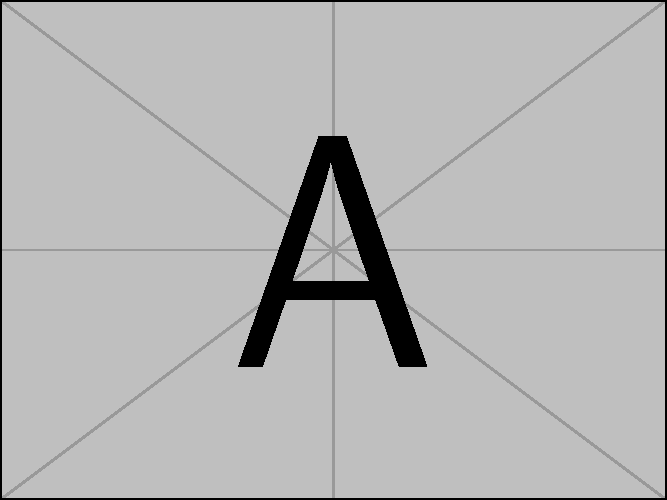
\includegraphics[width=0.3cm]{example-image-a}}]}]
\end{tikzpicture}
\begin{tikzpicture}
\duck[|stripes|={
      \stripes[height=1.0]}]
\end{tikzpicture}

\begin{tikzpicture}
\duck[|stripes|={
      \stripes[initialx=1]}]
\end{tikzpicture}
\begin{tikzpicture}
\duck[|stripes|={
      \stripes[initialy=0.8]}]
\end{tikzpicture}

\begin{tikzpicture}
\duck[|stripes|={
      \stripes[rotate=45]}]
\end{tikzpicture}
\begin{tikzpicture}
\duck[|stripes|={
      \stripes[rotate=-45]}]
\end{tikzpicture}
\end{tcblisting}

For more complex or multicoloured designs the stripes can easily be stacked on top of each other:
\begin{tcblisting}{title={multicoloured \texttt{stripes}}}
\begin{tikzpicture} 
\duck[tshirt=red, |stripes|={
\stripes[color=yellow, width=0.1]
\stripes[color=orange, width=0.1, initialx=0.0]}]
\end{tikzpicture}
\end{tcblisting}

\tcbset{righthand width=3cm}
A few examples to see \lstinline|stripes| in action:
\begin{tcblisting}{title={Inter duck}}
\definecolor{blueinter}{RGB}{0,102,170}%
\begin{tikzpicture}
\duck[tshirt=black,|stripes|={\stripes[color=blueinter]},football]
\end{tikzpicture}
\end{tcblisting}

\begin{tcblisting}{title={Juve duck}}
\begin{tikzpicture} 
\duck[tshirt=black,|stripes|={\stripes[color=white]},football]
\end{tikzpicture}
\end{tcblisting}

\begin{tcblisting}{title={Milan duck}}
\begin{tikzpicture}
\duck[tshirt=black,|stripes|={\stripes[color=red]},football]
\end{tikzpicture}
\end{tcblisting}

\begin{tcblisting}{title={M\"{o}nchengladbach duck}}
\definecolor{mggreen}{RGB}{37,166,89}%
\begin{tikzpicture} 
\duck[tshirt=mggreen,|stripes|={\stripes},football]
\end{tikzpicture}
\end{tcblisting}

\begin{tcblisting}{title={Palmeiras duck}}
\definecolor{verdep}{RGB}{0,100,55}%
\begin{tikzpicture} 
\duck[tshirt=green,jacket=verdep,football] 
\end{tikzpicture}
\end{tcblisting}

\begin{tcblisting}{title={Cagliari duck}}
\definecolor{rossocagliari}{RGB}{149,20,38}%
\definecolor{blucagliari}{RGB}{23,52,84}%
\begin{tikzpicture} 
\duck[tshirt=white, jacket=blucagliari,|stripes|={
\stripes[color=rossocagliari, width=0.46, distance=3]},football]
\end{tikzpicture}
\end{tcblisting}

\begin{tcblisting}{title={Sampdoria duck}}
\begin{tikzpicture} 
\duck[tshirt=blue, jacket=blue,|stripes|={
\stripes[color=white,rotate=-90,width=0.6,distance=1] 
\stripes[color=red,rotate=-90,width=0.2,distance=1.2] 
\stripes[color=black,rotate=-90,width=0.1,distance=1.3]
},football]
\end{tikzpicture}
\end{tcblisting}

\begin{tcblisting}{title={Brescia duck}}
\begin{tikzpicture} 
\duck[tshirt=blue, jacket=blue,|stripes|={
  \stripes[color=white, rotate=-70, width=0.22,distance=1.1, initialy=0.01]
  \stripes[color=white, rotate=40, width=0.2, distance=1.8, initialy=1.0,initialx=0.285]
},football]
\end{tikzpicture}
\end{tcblisting}

\section{Examples}

To see more examples of what can be done with the \tikzducks, you are invited to visit \url{https://github.com/samcarter/tikzducks}. 

If you have created a duck you would like to share with the community, I would be happy to add it to this collection, just make a pull request or open an issue in the bug tracking system.

\clearpage
\printindex

\end{document}
